\section{Experimental Evaluation}\label{sec:exp}
We evaluate our techniques on two real-world datasets, i.e., \pt{} and \sz{} in this section.
The trajectory dataset of \pt{}~\cite{pt} has 2.39 million of taxi trajectories, 75.67 million of GPS points in total, its maximum trajectory length is 3,490 GPS points.
The trajectories in \pt{} cover several cities around the Porto and has been cleaned for further analysis.
\sz{}~\cite{sz} includes 3.07 million of taxi trajectories with 53.53 GPS points, the maximum trajectory in it has 2,268 GPS points.

In Section~\ref{sec:case}, we evaluate the effectiveness of our proposal by the case studies on \pt{} and \sz{} trajectory dataset, respectively.
We then conduct a user study to demonstrate the superiority of our proposal in three real world applications in Section~\ref{sec:user}.
We perform a qualitative evaluation in Section~\ref{sec:quality} at last.
We conducted all experiments on a machine with Intel i7-8700, 3.2 GHertz CPU, 24 GBytes memory and NVIDIA GeForce GTX1080, 8 GHertz VRAM GPU, running on Windows 10.
We implemented all methods in Java 1.8. The methods call on the Processing 3~\cite{p3} for rendering.


\subsection{Case Study}\label{sec:case}

We demonstrate the effectiveness of our proposal by the case studies in \pt{} in Section~\ref{sec:pt} and \sz{} {in Section~\ref{sec:sz}}.
%In this section, we evaluate our method by presenting the applications on two taxi trajectory datasets: Porto and Shenzhen. We compare the visualizations generated by the full dataset, random sampling and the proposed method from multiple levels of details.

\subsubsection{Case Studies on \pt{}}\label{sec:pt}

\begin{figure*}[t]
	\centering
	\includegraphics[width=0.85\textwidth]{pictures/experiment_study/case_porto.pdf}
	\vspace{-3mm}
	\caption{Effectiveness studies of $\avats$ at dense and sparse regions with detail visualizations in \pt{}.}
	\label{fig:porto}
    \vspace{-6mm}
\end{figure*}

We first refer the cases in Fig.~\ref{fig:teaser} to elaborate the effectiveness of our proposal from the following three aspects.

\stitle{Effect of approaches with different zoom-levels}
Considering zoom level 11, Fig.~\ref{fig:teaser}(A) is the visualization result of full \pt{} trajectory dataset.
Given the sampling rate $\alpha = 1\%$, Fig.~\ref{fig:teaser}(C) and (E) visualized the returning results of uniform random sampling algorithm ($\rand$, see Algorithm~\ref{alg:rand})
and our advanced visual fidelity guaranteed sampling approach ($\avats$, see Algorithm~\ref{alg:plus}), respectively.
Obviously, Fig.~\ref{fig:teaser}(E) looks much more closer to Fig.~\ref{fig:teaser}(A) when comparing with Fig.~\ref{fig:teaser}(C).
In particular, our proposed $\avats$ not only preserves the visual structure of the full dataset,
but also shows the details of these cities which are far away from the center, as the dashed cycles shown in Fig.~\ref{fig:teaser}(E).
However, the details of these dashed cycles in Fig.~\ref{fig:teaser}(C), i.e., the returning result from $\rand{}$, are lost.
This issue turns more serious when we zoom in to the details of the visualization results.
Fig.~\ref{fig:teaser}(H) and (I) are the visualization result of $\rand$ and $\avats$  (with color encoding) at zoom level 15 with sampling rate $\alpha=1\%$.
Comparing with the visualization result of full dataset at such level, as shown in Fig.~\ref{fig:teaser}(G),
the $\rand{}$ in Fig.~\ref{fig:teaser}(H) only returns few trajectories and many information in raw data are lost.
Surprisingly, our $\avats$ in Fig.~\ref{fig:teaser}(I) captures the main sketch of the full dataset, even with more clear details with the help of color encoding.

\stitle{Effect of sampling rate}
We then evaluate the effect of sampling rate in different approaches.
Fig.~\ref{fig:teaser}(B) and (C) are the visualization results of $\rand{}$ with sampling rate $0.1\%$ and $1\%$, respectively.
Fig.~\ref{fig:teaser}(D) and (E) visualized the returning trajectory sets of our $\avats{}$ with sampling rate $0.1\%$ and $1\%$, respectively.
We then have the following observations:
(i) the larger sampling rate, the better visual fidelity of the visualization results, e.g.,
Fig.~\ref{fig:teaser}(C) and (E) are more closer to Fig.~\ref{fig:teaser}(A) when comparing with Fig.~\ref{fig:teaser}(B) and (D), respectively;
(ii) the visualization result of $\avats$ with sampling rate $0.1\%$ in Fig.~\ref{fig:teaser}(D)
performs even more better than the result of $\rand{}$ with sampling rate $1\%$ in Fig.~\ref{fig:teaser}(C) to capture the visual structure of the full dataset in Fig.~\ref{fig:teaser}(A).


\stitle{Effect of color encoding}
Next, we present the superiority of color encoding scheme in $\avats$, which denotes as $\cavats$ in subsequent sections.
Given zoom level 11 and sampling rate $1\%$, Fig.~\ref{fig:teaser}(E) and (F) are the visualization results of our $\avats$ and $\cavats$ (i.e., $\avats$ with color encoding), respectively.
It is worth to point out the visual clutter in the visualization result of full dataset is serious, as the embedded rectangle shown in Fig.~\ref{fig:teaser}(A).
It also exists in the result of $\avats$, see the embedded rectangle in Fig.~\ref{fig:teaser}(E).
However, the visualized result of $\cavats$ in Fig.~\ref{fig:teaser}(F) reduces the visual clutter in Fig.~\ref{fig:teaser}(A) and (E) successfully.
%The embedded rectangle in Fig.~\ref{fig:teaser}(F) visualized the result of $\avats$ with color encoding.
Obviously, it provides clear visual structure of the input dataset.
In addition, the comparison of the visualized results in Fig.~\ref{fig:teaser}(G) and (I) confirms the effectiveness of our proposed color encoding scheme for visual clutter in large dataset again.

We next present the effectiveness of our proposals with different detail views by investigating three regions of interest in \pt{}, as R1, R2, and R3 shown in Fig.~\ref{fig:porto}(A).

% Comments for revise figure: change the current order, R3 first, then R2, last R1 (current order), I am writing in update order, but ask Qiaomu update the figures with the new order.
% h -> a, i -> b
\stitle{Sparse region R1}
R1 is a sparse region and has few trajectories, as the visualization result of full \pt{} dataset shown in Fig.~\ref{fig:porto}(B1).
The reason is the two cities Paredes and Penafiel in R1 are far away from the center of Porto.
Given sampling rate $\alpha=0.5\%$, Fig.~\ref{fig:porto}(B2), (B3) and (B4) are the visualization results of the returning trajectory set from $\rand{}$, $\vats$ and $\avats$ with $\delta=64$, respectively.
As our above statement, the result of $\rand$ almost misses all information in sparse region.
While $\vats$ performs much better than $\rand$ as it provides theoretical visual fidelity guarantee, but it still lost detail information.
Taking Fig.~\ref{fig:porto}(B1) as reference, the trajectory bundle and trajectory structure are lost in Fig.~\ref{fig:porto}(B3$a$) and (B3$b$).
As expected, our advanced approach $\avats$ in Fig.~\ref{fig:porto}(B4) with perception tolerance value $\delta=64$ did an excellent job to capture the details in the full dataset when comparing with $\vats$ in Fig.~\ref{fig:porto}(B3).
As shown in Fig.~\ref{fig:porto}(B4$b$), the trajectory sketch of Penafiel is almost the same as it in Fig.~\ref{fig:porto}(B1$b$), the visualized result of full dataset.


\begin{figure*}[t]
	\centering
	\includegraphics[width=0.85\textwidth]{pictures/experiment_study/case_shenzhen.pdf}
	\vspace{-4mm}
	\caption{Case studies on \sz{} taxi trajectory dataset, sampling rate $\alpha = 1\%$.}
	\label{fig:shenzhen}
    \vspace{-3mm}
\end{figure*}

\stitle{Median region R2} It is near to the center of Porto, which has more taxi trajectories than R1, see Fig.~\ref{fig:porto}(A).
As noted in Fig.~\ref{fig:porto}(C1), R2 includes three cities: Ermesinde, Rio Tinto and Valongo.
Fig.~\ref{fig:porto}(C2) and (C3) visualized the returning result of $\avats$ with perception tolerance value $\delta=4$ and $64$, respectively.
Visually, Fig.~\ref{fig:porto}(C3) has more trajectory branch details than Fig.~\ref{fig:porto}(C2), as the rectangles $c$ and $d$ shown in them.
%It shows that the larger perception tolerance value, the more details in this region reserved at zoom level 14.
%Comparing with Fig.~\ref{fig:porto}(C3),
Fig.~\ref{fig:porto}(C4) is the result of $\cavats$, i.e., it colors the trajectories by their representativeness.
Intuitively, Fig.~\ref{fig:porto}(C4) shows its superiority over Fig.~\ref{fig:porto}(C3) to capture the trajectory distributions.
For example, the color of the region $f$ in Fig.~\ref{fig:porto}(C4) is {darker} than the rest two regions $e$ and $g$.
Thus, we can conclude Rio Tinto (region $f$) has more taxi trajectories than other two cities, which is hard to be concluded via Fig.~\ref{fig:porto}(C3), even Fig.~\ref{fig:porto}(C1), the visualization result of full dataset.
It verified that the color encoding scheme could enrich the visual information in large trajectory visualization.

\stitle{Dense region R3} It is the center of Porto, which has the highest concentration of the trajectories and causes serious visual clutter, as visualized in Fig.~\ref{fig:porto}(D1).
For example, the structure of trajectories in Fig.~\ref{fig:porto}(D1$i$) is unclear.
$\avats$ with $\delta=4$ alleviates the visual clutter and preserves the trajectory distribution, see Fig.~\ref{fig:porto}(D2).
Fig.~\ref{fig:porto}(D3) visualized the result of $\avats$ with $\delta=64$, which enhances the visual fidelity of Fig.~\ref{fig:porto}(D2).
Specifically, it preserves more details (see rectangle $h$) and has a more clear structure in the {densest} region (see rectangle $i$).
Visually, Fig.~\ref{fig:porto}(D4) is the best among these four visualization results.
It confirms the advantages of color encoding scheme in $\cavats$.

%$\avats$($delta = 4$) greatly alleviates the visual clutter and preserves the framework which basically follows the road network as shown in Fig.~\ref{fig:porto}(B$_2$).
% Furthermore, when setting the interpretation tolerance parameter $delta$ as 64, the structure is more clear as shown in region b of Fig.~\ref{fig:porto}(B$_3$,B$_4$),
%  and have more trajectory details than $\avats$($delta = 4$) as shown in region $a$ of Fig.~\ref{fig:porto}(B$_2$,B$_3$).
%  The trajectories with color encoding further enhance the visualization thus the audiences can compare the traffic flow of two route more easily.


\vspace{-2mm}

\subsubsection{Case Studies on \sz}\label{sec:sz}
We further evaluate the effectiveness of our approaches by using the taxi trajectories in Shenzhen, China.
The \sz{} trajectory dataset has many different characteristics with \pt{}, e.g., trajectory distribution, city centers, and taxi move patterns.
We set sampling rate $\alpha=1\%$ and perception tolerance value $\delta = 64$ in this section.

\stitle{Overview of Shenzhen}
Fig.~\ref{fig:shenzhen}(A) is the visualization result of full \sz{} dataset at zoom level 11.
The dense regions in southern of Shenzhen, as the dashed circles shown in Fig.~\ref{fig:shenzhen}(A), are \emph{Baoan, Nanshan, Futian} and \emph{Luohu} districts,
which are the most prosperous commercial regions in this city.
The returning results of $\rand$, $\avats$ and $\cavats$ are visualized in Fig.~\ref{fig:shenzhen}(B), (C) and (D), respectively.
Not surprisingly,  the visualized result of $\rand$ in Fig.~\ref{fig:shenzhen}(B) is quite different from the full dataset in Fig.~\ref{fig:shenzhen}(A).
$\avats$ in Fig.~\ref{fig:shenzhen}(C) shows it superiority by capturing the overview of \sz{} dataset and even preserves the isolated trajectories,
as highlighted in left-upper corner of Fig.~\ref{fig:shenzhen}(C).
It owes to $\avats$ provides theoretical visual fidelity guarantees on the returning result set.
$\avats$ with color encoding $\cavats$ further improved the visual fidelity of $\avats$.
Specifically, both Fig.~\ref{fig:shenzhen}(A) and (C) are suffering from visual clutter seriously,
e.g., it is unable to recognize the main roads in the circles $a$ and $b$ as both are full with trajectories.
However, the result of $\avats$ with color encoding, as shown in Fig.~\ref{fig:shenzhen}(D), reduce the visual clutter perfectly.
For example, it is clear that the main roads of circle a and b are these roads with {darker} colors in Figure~\ref{fig:shenzhen}(D).

We then present the advantages of our $\avats$ in two representative areas, i.e., airport and North railway station, in \sz{} dataset.

\stitle{Airport in Shenzhen}
Comparing with visualization result of full dataset in Fig.~\ref{fig:shenzhen}(E),
the visualized result of $\rand$ in Fig.~\ref{fig:shenzhen}(F) only includes very few trajectories.
both $\avats$ and $\cavats$ (see Fig.~\ref{fig:shenzhen}(G) and (H)) reserve the major structure of the airport area excellent.
Moreover, $\cavats$ provides richer information by computing the representativeness of trajectories.
For example, the taxi trajectories which pass through G4 and G104 is more than that in Baoan Avenue.
The reason is that the colors of G4 and G104 is {darker} than Baoan Avenue, as highlighted in Fig.~\ref{fig:shenzhen}(H).

%the random sampling only preserves the trajectories pass through several routes with very high traffic flow(shown as Fig.~\ref{fig:shenzhen}(F)).  Both $\avats$ and $\avats$ with color encoding can visualize the trajectory structure very well. The $\avats$ with color encoding further enriches the information by encoding the trajectory with color. For example, we can observe that there are more trajectories passing through G4 and G104 than Baoan Avenue, which is hard to be discovered from the Fig.~\ref{fig:shenzhen}(E,F,G).

\stitle{North railway station in Shenzhen}
We next investigate the visualizations of the full dataset, uniform random sampling result set, and visual fidelity guaranteed sampling result set around North railway station of Shenzhen, which are shown from Fig.~\ref{fig:shenzhen}(I) to (L).
Interestingly, $\avats$ and $\cavats$ visualized the overpass near North railway state clearly, as circle $c$ shown in both Fig.~\ref{fig:shenzhen}(K) and (L).
Due to visual clutter, the overpass is not clear in Fig.~\ref{fig:shenzhen}(I), which visualized the full dataset.
It even disappeared in the visualized result of $\rand$ in Fig.~\ref{fig:shenzhen}(G).
Moreover, it is easy to compare the traffic flows in different roads via $\cavats$ visualization result.
For example, the road G94 has a higher road traffic flow than the Minzhi Avenue and Meilong Avenue, as different colors shown in Fig.~\ref{fig:shenzhen}(L).


%Similarly, in the region near to the Shenzhen North Railway Station, the visualization generated by $\avats$ can reveal some road structure such as the \QM{round entrance to the motorway} shown as region c in Fig.~\ref{fig:shenzhen}(K). With the color encoding, we can also easily discover that



\subsection{User Study}\label{sec:user}
In this section, we conduct an extensive user study on three real-world applications, i.e., region center identification, reachable route inspection, and traffic flow detection, to demonstrate the superiority of our proposal.
We present our user study setting in Section~\ref{sec:uset}, and analyze the user study results in Section~\ref{sec:uret}.

%To further evaluate the effectiveness of $\avats$ from the the audience perspective, we conducted formal user studies to compare how users perform the urban exploration tasks with visualizations generated by whole dataset, random sampling and $\avats$.


\begin{figure}[t]
	\centering
	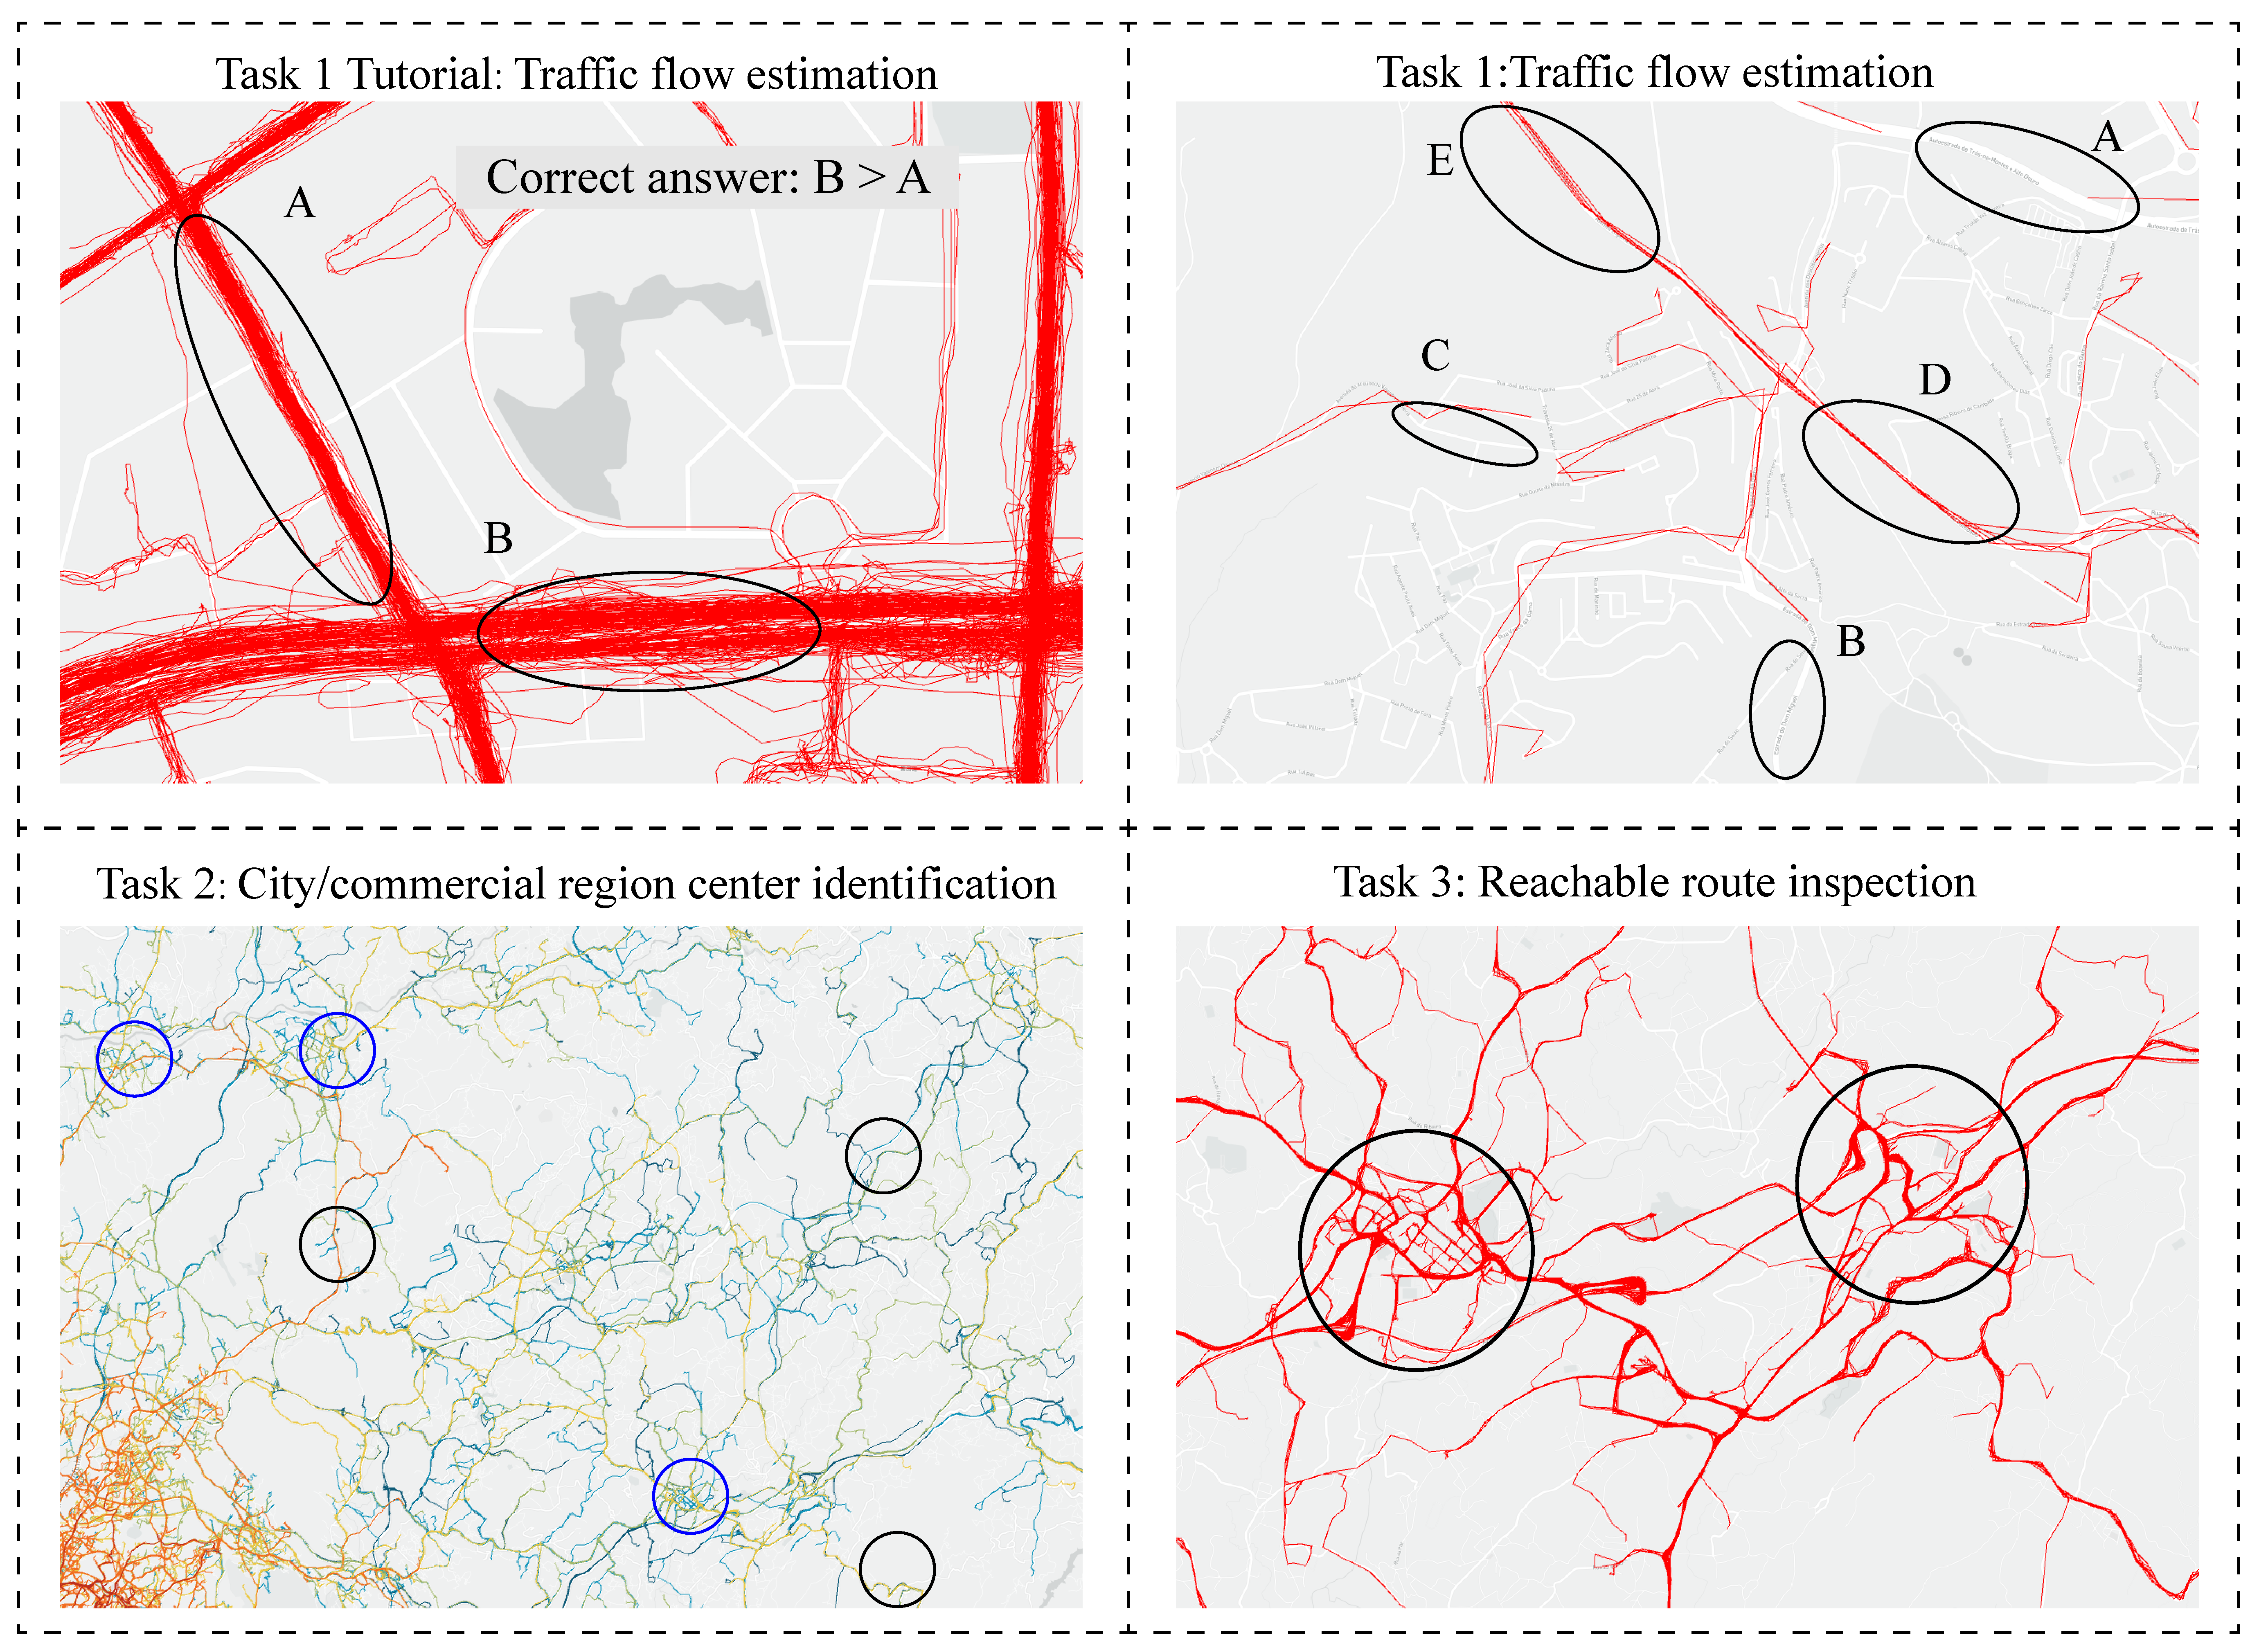
\includegraphics[width=0.48\textwidth]{pictures/user_study/interface.pdf}
	\caption{Three real-world applications in user study}
	\label{fig:apps}
\end{figure}

\subsubsection{User study setting}\label{sec:uset}

\stitle{Participants and apparatus}
We recruit 186 participants (24 females, 162 males, aged 18 to 29 with mean=21.16, standard derivation =1.48) with normal vision or normal corrected vision.
All participants have the background of computer science, 4.84\% of them have data visualization background.
The user study system is a web-based platform, which has the size-fixed interface and the participants perform the user study on their own  computers.
Considering the unfairness caused by different screen sizes, we recommend all participants to set the screen resolution as 1980*1080.
All images displayed on the interface have the same size 450*300.


\stitle{Studied visualization results}
We use the taxi trajectory dataset of \pt{} and \sz{} for the user study.
We study the visualization results which generated by different approaches in three real-world tasks.
We first introduce the studied data generation methods, then elaborate the tasks shortly.

The visualization results we investigated in user study are: (i) full dataset $\full$,
(ii) the result sets of $\rand$ (see Algorithm~\ref{alg:rand}),
(iii) the result sets of $\vats$ with performance optimizations (see Algorithm~\ref{alg:greedy}),
(iv) the result sets of $\avats$ without color encoding,
and (iv) the result sets of $\avats$ with color encoding (see Algorithm~\ref{alg:plus}), denotes as $\cavats$.
The sampling rate is $\alpha = 0.1\%$ and perception tolerance value $\delta = 64$ in all the visualization results in the user study section.
In each task, we use the identical regions with different visualized trajectories, which are returned from the above approaches.


\stitle{User study tasks}
All participants perform three tasks:  (T1) region center identification , (T2) reachable route inspection, and (T3) traffic flow estimation.
%as shown in Figure~\ref{fig:apps}(A), (B), and (C), respectively.

\sstitle{(T1) region center identification}
The center of the city or commercial region plays an important role in traffic management.
Consequently, the passing taxi trajectories of these centers are more than its surrounding regions, and results a star-shape cluster of trajectories in the visualization.
In this task, we randomly select 6 different regions which include city or commercial centers from \pt{} and \sz{}.
For each region, we ask the participate to identify the correct city/region center(s) in it.
As shown in Figure~\ref{fig:apps}(A), it asks the participate to identify 3 correct centers among these 6 cycles by clicking the corresponding cycles.
Specifically, T1 has 30 visualization views in total.
For each region of the visualization views,  we label the locations of the centers in it as the correct centers at first.
We then randomly select other areas which are not centers and far way from the correct centers, and label them as incorrect ones.
The number of correct centers in each visualization view is given to all participates.

%and remove these areas which too close to the correct ones,


% we have generated 145 visualizations(35 for T1, 75 for T2, 35 for T3) and 185 different questions(152 for T1, 21 for T2, 12 for T3).

\sstitle{(T2) reachable route inspection}
Intuitively, the visualized trajectories indicate the reachable routes of different regions.
In this task, we given a visualization view with two circular areas, as illustrated in Figure~\ref{fig:apps}(B),
then ask the participates to inspect the representative reachable routes between these two areas.
We assume the more trajectories in that route, the more representative it is.
For each visualization view, the number of reachable routes is given.
In T2, we randomly select 7 different regions which includes two or more cities/commercial districts.
In each region, we choose the identical two circular areas randomly for its 5 different visualization results.
%, which visualized the returned trajectory set of different approaches.


\sstitle{(T3) traffic flow comparison}
In practice, a road with large traffic flow has many passing trajectories, thus results to a denser and broader trajectory brunch in the visualization.
In the trajectory visualization with color encoding, such kind of pattern can also be highlighted by a concentration of trajectories with deep color.
It is important to preserve the traffic flow information during large trajectory visualization.
In this task, we ask the participates to compare the traffic flows in two roads by the given visualization results, as shown in Figure~\ref{fig:apps}(C).
In particular, the participants are asked to choose the road with large traffic flow by clicking the radio box.
They also can choose ``I am not sure'' if they cannot decided the answer.
T3 includes 5 randomly selected regions and each of them has clear road structure.
It has 25 visualization views and 60 road pair comparison in total.
We count the number of passing through trajectories in each road as the exact traffic flow in it.




%\textbf{T1. City/commercial region center identification.}
%% what participants do
%As shown by Figure~\ref{fig:user_study}(C), a visualization view was given and several regions were marked by circle. The participants needed to select the regions which could be city/commercial centers by click the corresponding circles. In each task, the number of correct regions were given.
%%Why possible
%The city or commercial region centers always have more passing trajectories from different directions than the surrounding regions, which results in the \UC{start-shape} cluster of trajectories in the visualization.
%%Generate the data
%To generate the test data of T1, we randomly chose several visualization views which contain city/commercial regions and labeled the locations of each city/commercial region center on the visualization as the correct locations first.  Then we randomly generated locations and remove the locations close to the correct locations, the remaining locations are the error locations. In each task of T1, with a given visualization, the same number of correct and wrong locations will be randomly selected.
%
%\textbf{T2. Reachable route inspection.}
%% what participants do
%Figure~\ref{fig:user_study}(D) shows the interface of T2, which includes a visualization and two circular regions. The users needed to draw several most representative reachable routes to connect the two regions. The number of the reachable routes is given.
%%Why possible
%The reachable routes indicate the routes connecting two regions, these routes must have the passing trajectories.
%%Generate the data
%To generate the test data, we randomly chose the visualization views which contain two or more city/commercial regions. In each task of T2, a visualization and two regions were randomly selected.

%\textbf{T3. Traffic flow estimation}.
%% what participants do
%As shown by Figure~\ref{fig:user_study}(B), with a given visualization, some road segments will be identified by ellipses(shown as~\ref{fig:user_study}(B)). Several road segment pairs were randomly selected and listed below the view. The participants were asked to choose the one with larger traffic flow by clicking the radio box. They can also choose ``I am not sure'' if they cannot decided the answer.
%%Why possible
%
%%Generate the data
%To generate the test data of T3,  we sampled and selected the visualization views which contain clear road structures. Then the number of trajectories passing through each road segment was counted as the traffic flow.



\stitle{User study procedure}
In the user study system, we first provide a brief introduction about the motivation, tasks and visual encoding scheme, then followed by three tasks.
In each task, we include a tutorial (with correct result) to help the participants familiarizing themselves with the interface, interaction and tasks.
For example, Figure~\ref{fig:apps}(D) shows a tutorial of T3 in Figure~\ref{fig:apps}(C), where the traffic flow in road A is smaller than it in road B, as the correct answer shown.
We then randomly choose different views with different questions in each task for different participates.
After she completed all the questions, her answers are collected and saved in the database for the result analysis.
At last, a post-interview were conducted to collect the feedback of the participants.
We refer the reviewers to our supplementary video for details of our user study procedure.

%The user study began with the introduction which introduces the motivation, tasks and visual encoding.
%Then the following sessions are divided into three blocks according to the task types. Each block starts with a task tutorial, in which the participants could perform several demo tasks, thus familiarizing themselves with the interface, interaction and tasks. For example, Figure~\ref{fig:user_study}(A) shows the demo task of T3, in which the users can check the correct answer after clicking the ``check'' button. After all the questions are finished, the answers and time usage are collected and saved in the database for the further analysis.

\subsubsection{User study result analysis}\label{sec:uret}
\TB{Figure~\ref{fig:accuracy} depicts the average accuracy of the different visualization approaches on different tasks from all user study participates.
Given a task with specified approach, we visualize the average accuracy of all questions by a colored circle and a line-segment to indicate the highest and lowest score of all questions of this task.}

\begin{figure}[t]
	\centering
	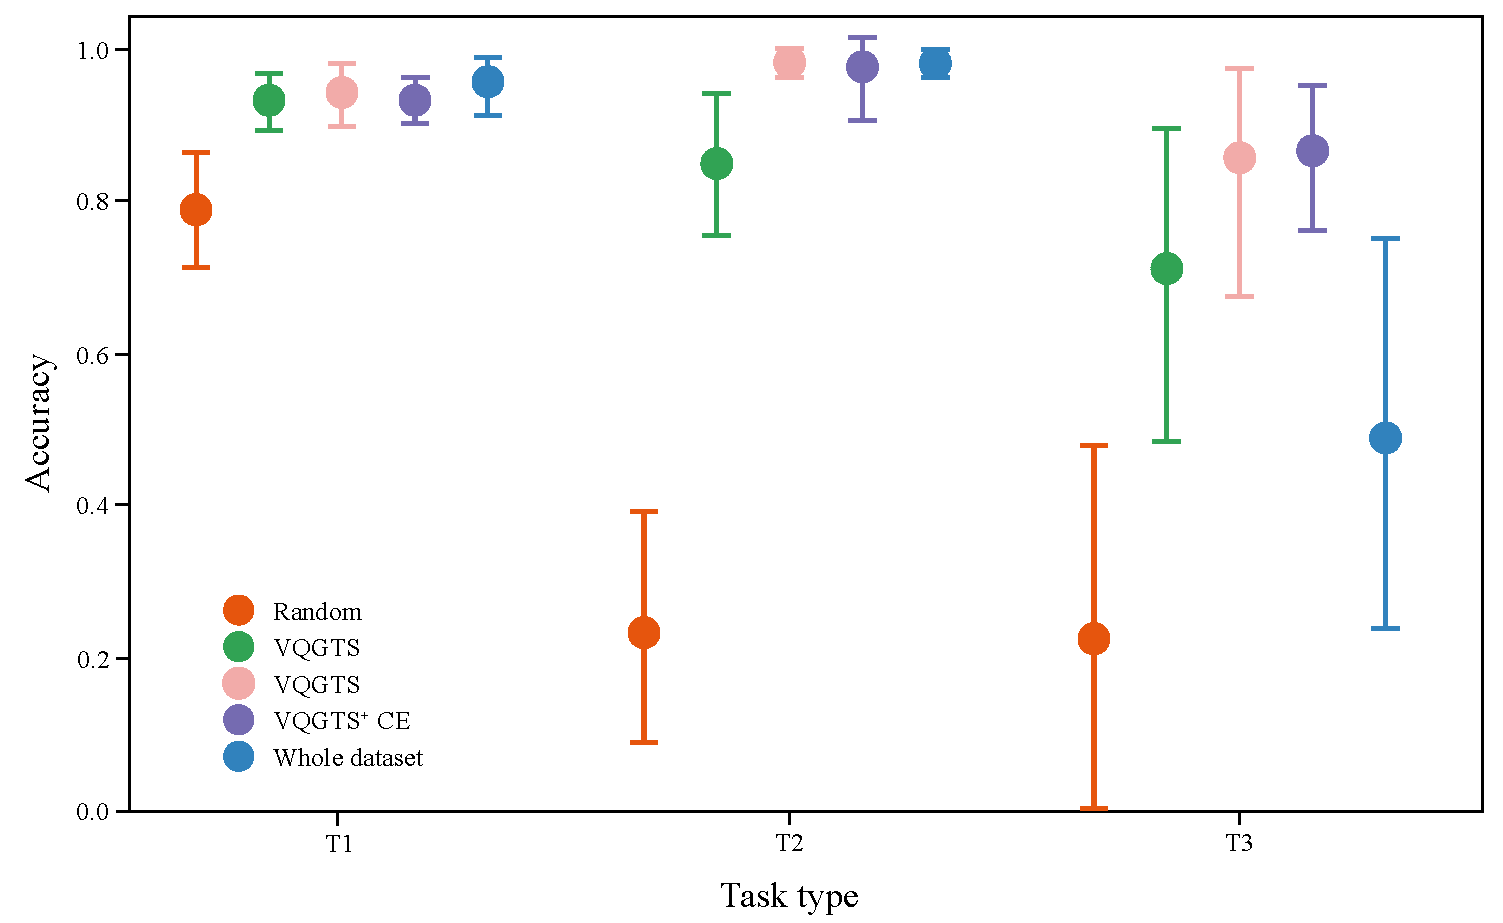
\includegraphics[width=0.44\textwidth]{pictures/user_study/accuracy.pdf}
	\caption{Average accuracy of three types of tasks. X axis indicates the task types. Y axis indicates the accuracy of different approaches.}
	\label{fig:accuracy}
\end{figure}



For T1 region center identification, the average accuracy of our proposed approaches (i.e., $\vats$, $\avats$, and $\cavats$) are higher than its of $\rand{}$ algorithm.
Moreover, our proposed approaches has a very close similar performance with visualizing the full dataset $\full$.
It means the visualized returning results of our proposed approaches worked as excellent as the full data visualization for the exploration of human activity center application.
We observed that the performance of $\cavats$ is slightly worse than performances of $\avats$ and $\full$.
In the post-interview, some of the participants say that the color of trajectories may distract user's attentions and make the cluster characteristics not obvious.


%the participants using all the three proposed methods had a very close performance with the participants using whole dataset, indicating the proposed methods can replace the whole dataset with a guaranteed performance in the exploration of human activity center with trajectory visualization.

For the reachable route inspection study in T2, it is no doubt the $\rand$ has the worst performance among these 5 visualization approaches as it lost many (if not all) detail information.
Unlike center identification in T1, the reachable route inspection in T2 are always performed at a fine-grained level of visualization,
which requires good preservation of the detail information, especially, for the sparse regions with few trajectories.
Thus, the advantages of our advanced approaches $\avats$ and $\cavats$ over $\vats$ become obvious and clear.
It owes to our advance approaches taken the data distribution and perception tolerance into consideration explicitly.
It also is worth to point out our $\avats$ (with average accuracy 0.968) outperforms the visualizations of $\full$ (with average accuracy 0.959) slightly.

%Interestingly,
%For the tasks of T2, $\avats$, $\avats$ with color encoding and the whole dataset all have similar accuracy scores which are far higher than random sampling.
%Moreover, $\avats$ and $\avats$ with color encoding also outperforms the $\vats$ clearly by taking the perception parameters into consideration.
% This results demonstrate the advantage of $\avats$ on the urban exploration at a detail level.


Visually, the task of traffic flow comparison in T3 are more difficult than T1 and T2.
It results in relative lower average accuracy for all approaches.  As expected, $\rand$ is the worst.
Interestingly, the average accuracy of visualization views of $\full$ is lower than our proposed approaches, i.e., $\vats,\avats$ and $\cavats$.
In the post-interview, the participants pointed out that many visualization views of $\full$ dataset had serious visual clutter,
which made it is impossible to compare the traffic flows in the two road segments.
The average accuracy of our proposed $\avats$ shows $\avats$ alleviated the visual clutter problem and preserved the clear structure.
$\cavats$ further highlighted the crowded road segments from the surroundings by color, which resulted it has the highest average accuracy in the task T3.

In summary, the qualitative user study of our proposal demonstrates the effectiveness of $\avats$ for large trajectory visualization by three real-world tasks.
All of our proposals ($\vats$, $\avats$, and $\cavats$) outperform the $\rand$ approach significantly.
In addition, the participates achieved equivalent or higher accuracy score in $\avats$ when comparing with the visualization of full dataset $\full$.


\subsection{Qualitative Evaluation}\label{sec:quality}
In this section, we conduct qualitative evaluation of our proposals on \pt{} and \sz{} trajectory datasets from two aspects: (i) the visual fidelity in different zoom levels,
and (ii) the running time with different sampling rates.

\begin{figure}
 \centering
 \small
 \begin{tabular}{cc}
   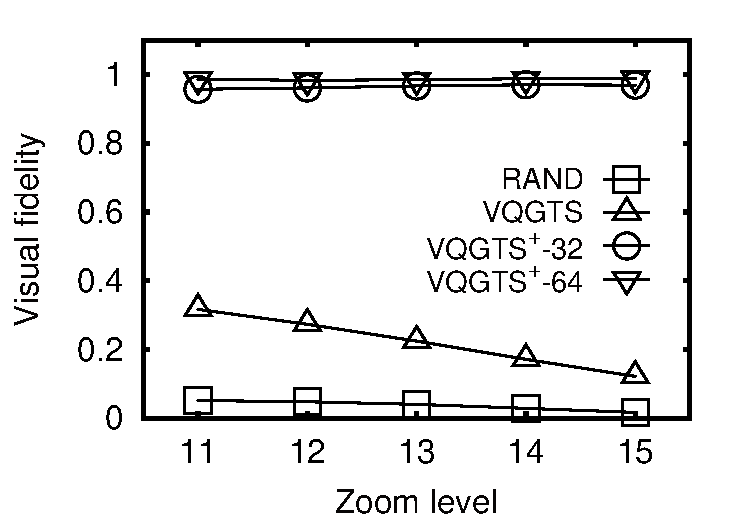
\includegraphics[width=0.48\columnwidth]{fporto}
   &
   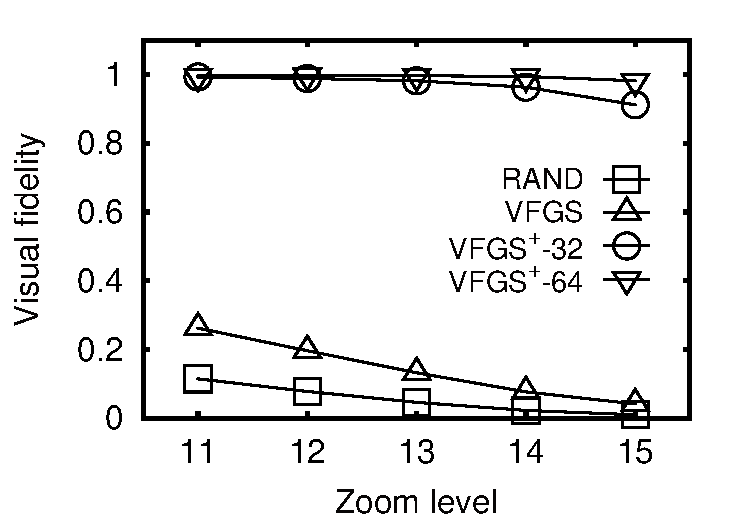
\includegraphics[width=0.48\columnwidth]{fshenzhen}
   \\
   (A) \pt{}
   &
   (B) \sz{}
 \end{tabular}
 \caption{Visual fidelity of proposed approaches}
 \label{fig:fidelity}
 \vspace{-4mm}
\end{figure}

\stitle{Visual fidelity evaluation}
We first evaluate the visual fidelity of our proposed methods.
We measure the visual fidelity of different approaches over the full dataset $\full$ by using the $loss()$ function we defined in Section~\ref{sec:def}.
Figure~\ref{fig:fidelity} (A) and (B) shows the visual fidelity of $\rand$, $\vats$, $\avats$ with $\delta=32$ and $\avats$ with $\delta=64$ from zoom level 11 to 15 in
\pt{} and \sz{}, respectively.
We can conclude that: (i) $\rand$ approach did not guarantee the visual fidelity of the result;
(ii) even $\vats$ offers theoretical visual fidelity guarantee w.r.t. the optimal sampled result set with given sampling rate, but it still has room for improving over the $\full$ dataset;
(iii) $\avats$ with $\delta=32$ and $\delta=64$ has excellent visual fidelity w.r.t. the $\full$ dataset. The minimum visual fidelity value is 0.95 and 0.91 in \pt{} and \sz{}, respectively.
It also confirms the superiority of our proposal;
and (iv) the visual fidelity of $\avats$ falls with the rising of zoom levels, e.g., from zoom level 11 to 15.
The reason is the higher zoom level, the more detail information are required.


\begin{figure}
 \centering
 \small
 \begin{tabular}{cc}
   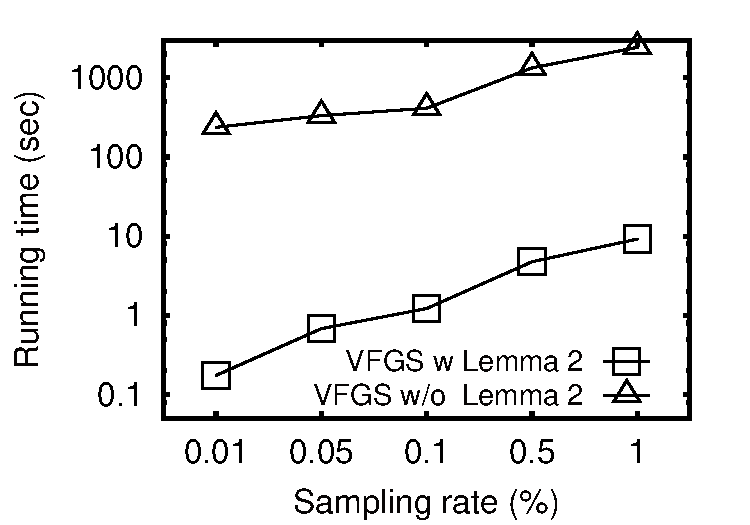
\includegraphics[width=0.48\columnwidth]{tporto}
   &
   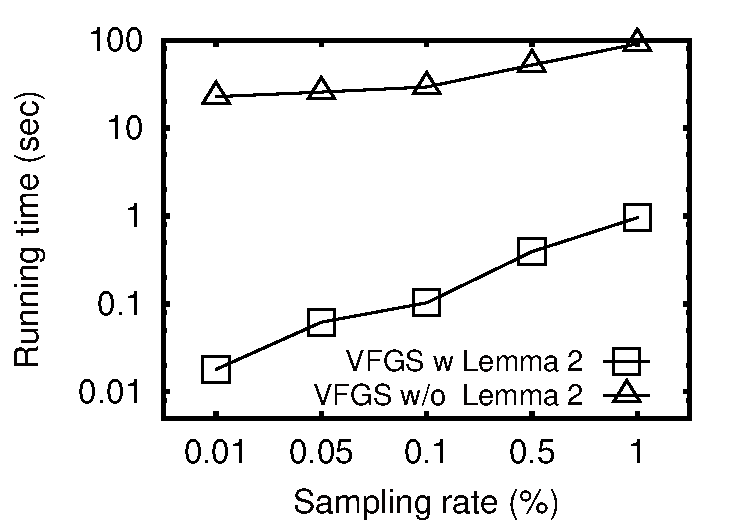
\includegraphics[width=0.48\columnwidth]{tshenzhen}
   \\
   (A) \pt{}
   &
   (B) \sz{}
 \end{tabular}
 \caption{The running time of $\vats$ with or without optimization techniques}
 \label{fig:cost}
 \vspace{-4mm}
\end{figure}


\stitle{Running time evaluation}
Last, we report the running time of our $\vats$ on two datasets: \pt{} and \sz{} by varying the sampling rate from $0.01\%$ to $1\%$.
It is no doubt our visual fidelity guaranteed sampling approach $\vats$ is quite slow without the performance optimizations in Section~\ref{sec:opt}.
Our optimized $\vats$ (e.g., $\vats$ with Lemma~\ref{lem:submodular}) outperform $\vats$ by one to three orders of magnitudes in both \pt{} and \sz{}, as shown in Figure~\ref{fig:cost}(A) and (B).
Finally, with excellent performance of our $\vats$, we conclude that our proposals provide interactive visualization for large trajectory data exploration, i.e., generate visualization results within seconds.





%\stitle{Overview of the Porto Distinct}
%Figure~\ref{fig:teaser}(A) presents the visualization generated by the whole dataset, from which we can get an overview of the movement patterns in Porto district. For example, large number of trajectories are concentrated in the center of the figure(shown around Figure~\ref{fig:teaser}(A$_1$)), indicating that the most taxi activities are around the \UC{Porto City}. In addition,
%many trajectory clusters distributed across the land, which indicates the locations of other cities in Porto district(shown as the dashed circle in Figure~\ref{fig:teaser}(A)).
%
%We compare the $\avats$ with \textit{uniform random sampling} at the overview.
%Figure~\ref{fig:teaser}(C,E) show the visualization generated by uniform random sampling and $\avats$ respectively. Both of these two sampling methods take 0.01 as the sampling rate. The uniform random sampling almost only preserves the visual structure around the Porto City and the trajectories at the marginal regions are lost.
%The visualization generated by $\avats$ looks close to the whole dataset. Not only the \UC{Porto City} but also the marginal city structures are well preserved, which are shown as the dash circles in Figure~\ref{fig:teaser}(E).
%
%Furthermore, the color encoding further enhances the visualization by revealing the \QM{representativeness} of the trajectories.
%As shown by the rectangle region in Figure~\ref{fig:teaser}(E), there is no clear pattern that can be discovered due to the dense concentration of massive trajectories. While in the same region of Figure~\ref{fig:teaser}(F), some trajectories with high representative scores are highlighted by dark orange color such as F$_1$, which indicates Avenida da Boavista, a main avenue in Porto City.
%%From the overview, $\avats$ can preserve the general structure very well in the comparison with uniform random sampling, and more information of the movement can be visualized with color encoding.
%
%
%An important factor affecting the visual fidelity of sampling results is the sampling rate. Figure~\ref{fig:teaser}(C,B) show the sampling results of random method with sampling rate set as 0.01 and 0.001. With the decreasing of the sampling rate, the shape of the trajectory visualizations clearly shrink to the Porto City and result to the loss of visual fidelity at the marginal region. Figure~\ref{fig:teaser}(E,D) demonstrate the visualization of $\avats$ with the sampling rate of 0.01 and 0.001. We observe that when the sampling rate is decreased, the overview framework of the trajectories remains the same but the trajectories around Porto City are significantly removed since more \QM{blank space/gap} can be found around the Porto City as shown in the rectangle of Figure~\ref{fig:teaser}(D).


%\begin{figure}[t]
%	\centering
%	\vspace{2mm}
%	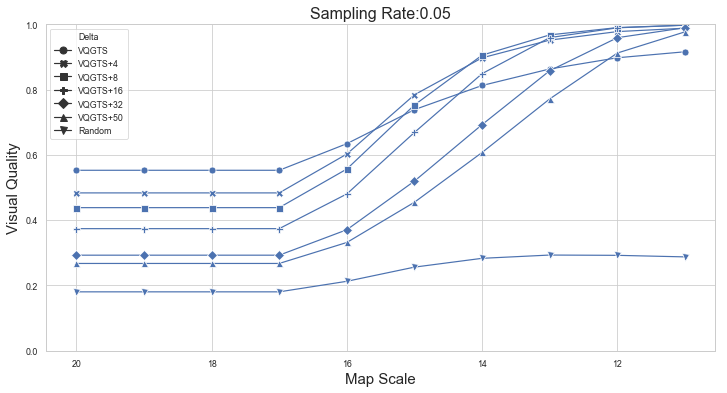
\includegraphics[width=0.45\textwidth]{pictures/experiment_study/quanlity.png}
%	\caption{Visual quality chart. X axis indicates map scale from detail view to overview; y axis indicate the visual quality. }
%	\vspace{0mm}
%	\label{fig:quality_chart}
%\end{figure}



%Figure~\ref{fig:shenzhen}(A-D) present the overview visualization generated by whole dateset, random sampling, $\avats$ and $\avats$ with color encoding at the top level. The visualization of raw dataset(Figure~\ref{fig:shenzhen}(A)) shows the there are several dense trajectory clusters in southern districts of Shenzhen, including \textit{Baoan}, \textit{Nanshan}, \textit{Futian} and \textit{Luohu} districts, which are the most prosperous commercial zones of Shenzhen. Figure~\ref{fig:shenzhen}(B) presents the trajectories generated by random sampling. We observe that the most of the trajectories sampled by random sampling are located at the commercial zones. On the other hand, the trajectories at the north Shenzhen are missing, thus making the visualization visually different from the whole dataset.
%$\avats$ outperforms random method by guaranteeing the spatial coverage of the whole trajectories thus result in a higher visual fidelity. Further more, some isolate trajectories are still preserved shown in Figure~\ref{fig:shenzhen}(C). $\avats$ with color is able to reveal the spatial distribution of the trajectories. For example, for the regions a, b in Figure~\ref{fig:shenzhen}(A or C), the visualization is unable to explain which region has more taxi activities because both of these two regions are fully covered by trajectories. In Figure~\ref{fig:shenzhen}(D), we find the more trajectories encoded by deep color are found in region a than that of region b, which indicates more trajectories can be found in region a than region b.

%We further evaluate the proposed approach using the taxi trajectories of Shenzhen, a booming city in the southern China and has very different urban form from Porto District. The dataset we used includes 428K taxi trajectories collected from \QM{**} taxis in one day. All the visualization generated by the sampling methods which sets the sampling rates as 0.01. 